\section{Dynamic Programming and the Linear Quadratic Regulator}

\subsection{The Optimal Control Problems}

In this section, we will outline the deterministic continuous-time optimal control problem that we will aim to solve. We will denote the state at time $t$ as $\st(t) \in \R^n$, and the control as $\ac(t) \in \R^m$. We will also occasionally write these as $\st_t$ and $\ac_t$, respectively. We will write the continuous-time systems dynamics as 
\begin{equation}
    \stdot(t) = \bm{\f}(\st(t),\ac(t),t).
    \label{eq:2_ct_dyn}
\end{equation}
We will refer to a history of control input values during an interval $[t_0,t_f]$ as a control history, and we will refer to a history of state values over this interval as a state trajectory. 

Different control problems may call for various constraints. For example, we may constrain a quadrotor to only fly in space not occupied by obstacles. Examples of constraints we will see are
\begin{itemize}
    \item Initial and final conditions, $\st(t_0) = \st_0$, $\st(t_f) = \st_f$
    \item Trajectory constraints, $\munderbar{\st} \leq \st(t) \leq \bar{\st}$
    \item Control limits, $\munderbar{\ac} \leq \ac(t) \leq \bar{\ac}$.
\end{itemize}
A state trajectory and control history that satisfy the constraints during the entire time interval $[t_0,t_f]$ are called admissible trajectories and admissible controls, respectively. 

Finally, we will define the performance measure, 
\begin{equation}
    J = \cost_f(\st(t_f),t_f) + \int_{t_0}^{t_f} \cost(\st(t),\ac(t),t) dt
    \label{eq:2_perf}
\end{equation}
where $\cost$ is the instantaneous cost function, and $\cost_f$ is the terminal state cost. We are now able to state the continuous-time optimal control problem. 
We aim to find an admissible control, $\ac^*$, which causes the system (\ref{eq:2_ct_dyn}) to follow an admissible trajectory, $\st^*$, that minimizes the performance measure given by (\ref{eq:2_perf}). The minimizer $(\st^*,\ac^*)$ is called an optimal trajectory-control pair. 

Note, first of all, that this is an extremely general problem formulation. We have not fixed our system dynamics, cost function, or specific constraints. We can't, in general, guarantee the existence or uniqueness of the optimal solution. 

There are two possible solution forms for the optimal control. The first, $\ac^* = e(\st(t_0),t)$ is referred to as an open-loop solution. This is an input function that is applied to the system, without using feedback. Practically, such solutions usually require augmentation with a feedback controller, as small model mismatch may lead to compounding errors. The second possible solution form is a feedback policy, $\ac^* = \pol(\st(t),t)$. This feedback law maps all state-time pairs to an action and thus is usually more robust to possible model mismatch. However, depending on the particular problem formulation, open-loop solutions may be easier to compute. 
% add discussion of discrete time optimal control problem?

\subsection{Dynamic Programming and the Principle of Optimality}


\begin{figure}[t]
    \centering
    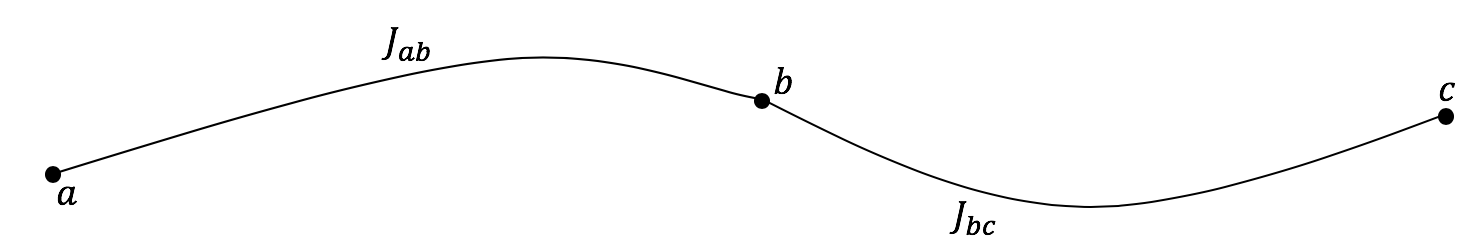
\includegraphics[width=0.8\linewidth]{figs/optimality.png}
    \caption{An optimal trajectory connecting point $a$ to point $c$. There are no better (lower cost) trajectories than the sub-trajectory connecting $b$ and $c$, by the principle of optimality.}
    \label{fig:opt1}
\end{figure}

In this chapter we will outline the principle of optimality, and the method of dynamic programming (DP), one of two main approaches to solving the optimal control problem. The second, so-called variational approaches based on Pontryagin's Maximum Principle (PMP) will be discussed in future chapters. Dynamic programming has the strong advantage of yielding a feedback policy, however, exactly solving the dynamic programming problem is infeasible for many systems. We will address special cases in which the DP problem can be solved exactly, and approximate methods that work for a wide variety of systems. 

Despite having just introduced the optimal control problem in continuous time, we will be operating in discrete time here, in which we aim to minimize 
\begin{equation}
    \J_f(\st_0) = \cost_f(\st_N) + \sum_{k=0}^{N-1} \cost(\st_k, \ac_k, k).
    \label{eq:disc_cost}
\end{equation}
We will extend the methods we develop in this chapter to continuous time in the next chapter. 

The principle of optimality is as follows. Figure \ref{fig:opt1} shows a trajectory from point $a$ to $c$. If the cost of the trajectory, $J_{ac} = J_{ab} + J_{bc}$, is minimal, then $J_{bc}$ is also a minimum cost trajectory connecting $b$ and $c$. The proof of this principle, stated informally, is simple. Assume there exists an alternative trajectory connecting $b$ and $c$, for which we will write the cost as $\tilde{J}_{bc}$, that achieves $\tilde{J}_{bc} < J_{bc}$. Then, we have 
\begin{align}
    \tilde{J}_{ac} &= J_{ab} + \tilde{J}_{bc}\\
    &< J_{ab} + J_{bc}\\
    &= J_{ac},
\end{align}
and thus $J_{ac}$ isn't minimal. More formally,

\begin{theorem}[Discrete-time Principle of Optimality]
Let $\pi^* = (\pi_0^*, \ldots, \pi^*_{N-1})$ be an optimal policy. Assume state $\st_k$ is reachable. Consider the subproblem whereby we are at $\st_k$ at time $k$ and we wish to minimize the cost-to-go from time $k$ to time $N$. Then the truncated policy $(\pi_k^*, \ldots, \pi^*_{N-1})$ is optimal for the subproblem.
\end{theorem}

Dynamic programming, intuitively, proceeds backwards in time, first solving simpler shorter horizon problems. If we have found the optimal policy for times $k+1$ to $N-1$, along with the associated cost-to-go for each state, choosing the optimal policy for time $k$ is a one step optimization problem. More concretely, we will assume we have dynamics of the form $\st_{k+1} = \f(\st_k,\ac_k,k)$ with $\ac_k \in \mathcal{U}(\st_k)$, and the cost given by (\ref{eq:disc_cost}). Then, dynamic programming iterates backward in time, from $N-1$ to $0$, with
\begin{align}
    \J_N(\st_N) &= \cost_T(\st_N)\\
    \J_k(\st_k) &= \min_{\ac_k \in \mathcal{U}(\st_k)} \left\{ \cost_k(\st_k,\ac_k,k) + \J_{k+1}(\f(\st_k,\ac_k,k)) \right\}.
    \label{eq:DP_rec}
\end{align}
Note that here we have considered only deterministic dynamical systems (there is no stochastic disturbance). 

Practically, dynamic programming raises many practical issues if one were to attempt to apply it directly. To perform the recursion, $\J_{k+1}$ must be known for all $\st_{k+1}$ (or more precisely, all $\st_{k+1}$ that are reachable from $\st_k$). If the state space is discrete (and relatively small), this is tractable as the cost-to-go may just be maintained in tabular form. In the next subsection, we will discuss an extremely important case in continuous space in which the cost-to-go can be computed exactly for all states. However, for general systems, we can not expect to be able to compute the cost-to-go for all states. Possible approaches to make the DP approach tractable are discretizing the state space, approximating the cost-to-go (i.e. restricting the family of functions that $\J_{k+1}$ may be in), or interpolating between cost-to-go computed for a finite set of states. 

% should talk about the limitations of each of these methods

% should talk about how this yields a globally optimal, closed-loop policy

% add discrete DP example 

\subsection{Discrete LQR}

An important instance in which dynamic programming can be solved analytically for continuous state-action systems is the \textit{linear quadratic regulator} problem. We will fix the dynamics of the system to be (possibly time-varying) linear, 
\begin{equation}
    \st_{k+1} = A_k \st_k + B_k \ac_k
\end{equation}
and the cost function is quadratic
\begin{align}
    \cost(\st_k, \ac_k) &= \frac{1}{2} ( \st_k^T Q_k \st_k + \ac_k^T R_k \ac_k )\\
    \cost_N(\st_k) &= \frac{1}{2} \st_k^T Q_N \st_k
\end{align}
where $Q_k \in \R^{n \times n}$ is positive semi-definite and $R_k \in \R^{m \times m}$ is positive definite for all $k = 0, \ldots, N$. Importantly, we assume $\st_k$ and $\ac_k$ are unconstrained for all $k$. To perform DP recursion, we initialize 
\begin{equation}
    \J_N^*(\st_N) = \frac{1}{2} \st_N^T Q_N \st_N \vcentcolon= \frac{1}{2} \st_N^T V_N \st_N.
\end{equation}
Then, applying (\ref{eq:DP_rec}), we have
\begin{equation}
    \J_{N-1}^*(\st_{N-1}) = \frac{1}{2} \min_{\ac_{N-1} \in \R^m} \left\{ \st_{N-1}^T Q_{N-1} \st_{N-1} + \ac_{N-1}^T R_{N-1} \ac_{N-1} + \st_N^T V_N \st_N \right\}
\end{equation}
which, applying the dynamics,
\begin{align}
\label{eq:LQR_rec_cost}
    \J_{N-1}^*(\st_{N-1}) = \frac{1}{2} \min_{\ac_{N-1} \in \R^m} & {\large\{} \st_{N-1}^T Q_{N-1} \st_{N-1} + \ac_{N-1}^T R_{N-1} \ac_{N-1}\\
    &+ (A_{N-1} \st_{N-1} + B_{N-1} \ac_{N-1})^T V_N (A_{N-1} \st_{N-1} + B_{N-1} \ac_{N-1}) {\large\}}. \nonumber
\end{align}
Rearranging, we have
\begin{align}
    \J_{N-1}^*(\st_{N-1}) = \frac{1}{2} \min_{\ac_{N-1} \in \R^m} {\large\{}
    & \st_{N-1}^T (Q_{N-1} + A_{N-1}^T V_N A_{N-1}) \st_{N-1}\\ \nonumber
    & + \ac_{N-1}^T (R_{N-1} + B_{N-1}^T V_N B_{N-1}) \ac_{N-1}\\\nonumber
    & + 2 \ac_{N-1}^T (B_{N-1}^T V_N A_{N-1}) \st_{N-1} \nonumber
    {\large\}}.
\end{align}
Note that this optimization problem is convex in $\ac_{N-1}$ as $R_{N-1} + B_{N-1}^T V_N B_{N-1} > 0$. Therefore, any local minima is a global minima, and therefore we can simply apply the first order optimality conditions. Differentiating,
\begin{equation}
    \frac{\partial \J_{N-1}^*(\st_{N-1})}{\partial \ac_{N-1}} = (R_{N-1} + B_{N-1}^T V_N B_{N-1}) \ac_{N-1} + (B_{N-1}^T V_N A_{N-1}) \st_{N-1}
\end{equation}
and setting this to zero yields
\begin{equation}
    \ac^*_{N-1} = - (R_{N-1} + B_{N-1}^T V_N B_{N-1})^{-1} (B_{N-1}^T V_N A_{N-1}) \st_{N-1}
\end{equation}
which we write
\begin{equation}
    \ac^*_{N-1} = L_{N-1} \st_{N-1}
\end{equation}
which is a time-varying linear feedback policy. Plugging this feedback policy into (\ref{eq:LQR_rec_cost}),
\begin{align}
    \J_{N-1}^*(\st_{N-1}) =& \st_{N-1}^T (Q_{N-1}  + L_{N-1}^T R_{N-1} L_{N-1} \\
    & + (A_{N-1} + B_{N-1} L_{N-1})^T V_N   (A_{N-1} + B_{N-1} L_{N-1})) \st_{N-1}. \nonumber
\end{align}
Critically, this implies that the cost-to-go is always a positive semi-definite quadratic function of the state. Because the optimal policy is always linear, and the optimal cost-to-go is always quadratic, the DP recursion may be recursively performed backward in time and the minimization may be performed analytically. 

Following the same procedure, we can write the DP recursion for the discrete-time LQR controller:
\begin{enumerate}
    \item $V_N= Q_N$
    \item $L_k = - (R_{k} + B_{k}^T V_{k+1} B_{k})^{-1} (B_{k}^T V_{k+1} A_{k})$
    \item $V_{k} = Q_{k}  + L_{k}^T R_{k} L_{k} + (A_{k} + B_{k} L_{k})^T V_{k+1}   (A_{k} + B_{k} L_{k})$
    \item $\ac^*_k = L_k \st_k$
    \item $\J^*_k(\st_k) = \frac{1}{2} \st_k^T V_k \st_k$
\end{enumerate}
There are several implications of this recurrence relation. First, even if $A,B,Q,R$ are all constant (not time-varying), the policy is still time-varying. Why is this the case? Control effort invested early in the problem will yield dividends over the remaining length of the horizon, in terms of lower state cost for all future time steps. However, as the remaining length of the episode becomes shorter, this tradeoff is increasingly imbalanced, and the control effort will decrease. 
However, for a linear time-invariant system, if $(A,B)$ controllable, the feedback gain $L_k$ approach a constant as the episode length approaches infinity. This time-invariant policy is practical for long horizon control problems, and may be approximately computed by running the DP recurrence relation until approximate convergence. 

\subsection{Iterative LQR and Differential Dynamic Programming}



\subsection{LQG}